\subsection{House names}
\label{subsec:application:building_the_model:house_names}

In the third step, something interesting finally happens. This step introduces the names for houses, or in model terms, the $\type{name}$ attribute on the $.\type{House}$ class is introduced, including its values. \cref{subsec:library_of_transformations:type_level_transformations:data_fields} is used to introduce the field, while on the instance level, \cref{subsec:library_of_transformations:instance_level_transformations:data_field_values} is used to introduce the values.

The $classtype$ of the new field is $.\type{House}$, as the field will be defined for houses. The $name$ of the new field is $\type{name}$ and the $fieldtype$ is $\type{string}$. The set of objects of which the value is set is is equal to all house objects, so $objects = \{TR, BHP\}$. The function for $obids$ returns the existing identifier of each of these objects. The $values$ function is defined as follows:
\begin{equation*}
    values = \{(TR, \text{``TwoRem''}), (BHP, \text{``B.H. Paleis''})\}
\end{equation*}

The following model is obtained:

\LTXtable{\textwidth}{tex/06_application/02_building_the_model/tables/03_house_names.tex}

\begin{figure}[p]
    \centering
    \begin{subfigure}{0.98\textwidth}
        \centering
        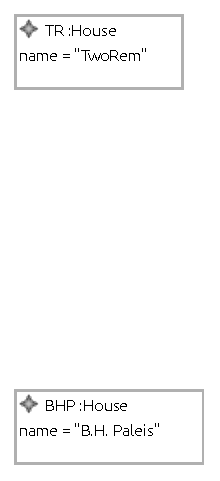
\includegraphics{images/06_application/instance_model/step03.pdf}
        \caption{Instance Model $Im_3$}
        \label{fig:application:building_the_model:house_names:ecore:instance_model}
    \end{subfigure}
    \\
    \begin{subfigure}{0.98\textwidth}
        \centering
        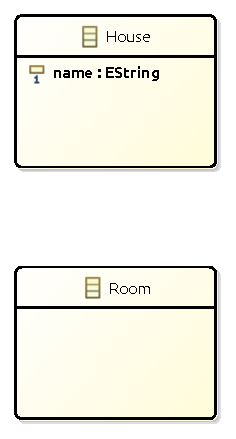
\includegraphics{images/06_application/type_model/step03.pdf}
        \caption{Type Model $Tm_3$}
        \label{fig:application:building_the_model:house_names:ecore:type_model}
    \end{subfigure}
    \caption{The Ecore model after step 3}
    \label{fig:application:building_the_model:house_names:ecore}
\end{figure}

\begin{figure}[p]
    \centering
    \begin{subfigure}{0.98\textwidth}
        \centering
        % To use this figure in your LaTeX document
% import the package groove/resources/groove2tikz.sty
%
\begin{tikzpicture}[scale=\tikzscale,name prefix=step03-]
\node[basic_node] (n0) at (2.680, -1.040) {\ml{\uline{\textit{BHP}} : \textbf{House}\\name = "B.H. Paleis"}};
\node[basic_node] (n1) at (2.660, -0.340) {\ml{\uline{\textit{TR}} : \textbf{House}\\name = "TwoRem"}};

\end{tikzpicture}

        \caption{Instance Graph $IG_3$}
        \label{fig:application:building_the_model:house_names:groove:instance_graph}
    \end{subfigure}
    \\
    \begin{subfigure}{0.98\textwidth}
        \centering
        % To use this figure in your LaTeX document
% import the package groove/resources/groove2tikz.sty
%
\begin{tikzpicture}[scale=\tikzscale,name prefix=step03-]
\node[basic_node] (n0) at (2.680, -1.040) {\ml{\uline{\textit{BHP}} : \textbf{House}\\name = "B.H. Paleis"}};
\node[basic_node] (n1) at (2.660, -0.340) {\ml{\uline{\textit{TR}} : \textbf{House}\\name = "TwoRem"}};

\end{tikzpicture}

        \caption{Type Graph $TG_3$}
        \label{fig:application:building_the_model:house_names:groove:type_graph}
    \end{subfigure}
    \caption{The GROOVE graphs after step 3}
    \label{fig:application:building_the_model:house_names:groove}
\end{figure}

A visual representation of $Tm_3$ and $Im_3$ can be found in \cref{fig:application:building_the_model:house_names:ecore}. Similarly, a visual representation of $TG_3$ and $IG_3$ can be found in \cref{fig:application:building_the_model:house_names:groove}. Please note that because of the definitions of $f_3(Im_3)$ and $f'_3(IG_3)$, we have that $f_3(Im_3) = IG_3$ and $f'_3(IG_3) = Im_3$. Furthermore, $f_3(Im_3)$ and $f'_3(IG_3)$ are valid mapping functions themselves, such that they can be combined with another mapping function in the next step.

Although visually the models are still not very advanced, formally they already from quite a definition. This definition will only get more substantial as more fields and objects are added in the next steps.

\afterpage{\FloatBarrier}